\begin{flushright} {\tiny {\color{gray} python\_codes/fieldstone\_119/text.tex}} \end{flushright}

\lstinputlisting[language=bash,basicstyle=\small]{python_codes/fieldstone_119/keywords}

\begin{center}

\fbox{\textbf{\huge \color{teal} P}}
Codes at \url{https://github.com/cedrict/fieldstone/tree/master/python_codes/fieldstone_01}
\end{center}

\par\noindent\rule{\textwidth}{0.4pt}

{\sl This fieldstone was developed in collaboration with Anthony Jourdon}. %\index{contributors}{J. Mos}

\par\noindent\rule{\textwidth}{0.4pt}
%%%%%%%%%%%%%%%%%%%%%%%%%%%%%%%%%%%%%%%%%%%%%%%%%%%%%%%%%%%%%%%%%%%%%%%%%%%%%%%%%%%%%%%%%%%%%%

\subsection*{About lithostatic pressure}

Let us look in section 2.2 of \textcite{tusc}:
``The normal force per unit area on horizontal planes increases linearly with
depth. The normal stress due to the weight of the overlying rock or over-
burden is known as the lithostatic stress or pressure.''

Also, on wikipedia\footnote{\url{https://en.wikipedia.org/wiki/Overburden_pressure}}:
``
Pressure is force magnitude applied over an area. Overburden pressure is a geology term that denotes the pressure caused by 
the weight of the overlying layers of material at a specific depth under the earth's surface.
Overburden pressure is also called lithostatic pressure, or vertical stress.
In a stratigraphic layer that is in hydrostatic equilibrium; the overburden pressure at a depth $z$, assuming the magnitude 
of the gravity acceleration is approximately constant, is given by: 
\[
P(z)=P_0 + g \int_0^z \rho(z) dz
\]
where $z$ is the depth in meters, $P(z)$ is the overburden pressure at depth $d$,
$P_0$ is the pressure at the surface, $\rho(z)$ is the density of the material above the depth $z$,
$g$ is the gravity acceleration in \si{\meter\per\square\second}.

In deep-earth geophysics/geodynamics, gravitational acceleration varies significantly over depth and $g$
should not be assumed to be constant, and should be inside the integral. ''

Finally, in Gerya's book:
``In geosciences, pressure is often considered as corresponding to the hydrostatic (litho-
static) condition everywhere and it is computed as a function of depth $y$ and vertical density
profile $\rho(y)$
\[
P(y)=P_0 + g \int_0^y \rho(y) dy
\]
where $P_0=0.1$~MPa is pressure on the Earth’s surface and $g$ is the gravitational
acceleration.''

On the AAPG wiki page\footnote{\url{https://wiki.aapg.org/Geostatic_and_lithostatic_pressure}}:
``The geostatic pressure at a given depth is the vertical pressure due to the weight of a column of 
rock and the fluids contained in the rock above that depth. Lithostatic pressure is the vertical 
pressure due to the weight of the rock only. ''

In conclusion there seems to be a widely accepted definition as to what lithostatic pressure is.
At a given location it is solely given as a function of the column of material 
above it. Since $\rho>0$ and $g>0$ too, the (absolute value of) the lithostatic pressure
can only increase with depth.

%--------------------------------------------------------
\subsection*{The numerical approach of Jourdon \& May (2022)}

What follows is based on \textcite{joma22} (2022) in which the authors present an
``efficient parallel method to compute lithostatic pressure in thermo-mechanical geodynamic models''.

We then start from 
\begin{equation}
-\vec\nabla p + \rho \vec{g} = \vec{0}
\label{eq:gradpstrong}
\end{equation}
and we take the divergence of this expression:
\[
\vec\nabla \cdot \vec\nabla p = \vec\nabla \cdot \rho \vec{g} 
\]
We multiply by a test function $q$ and integrate over the domain:
\[
\int_\Omega q \vec\nabla \cdot \vec\nabla p \;dV
=
\int_\Omega q \vec\nabla \cdot \rho \vec{g} \;dV
\]
We integrate by parts both LHS and RHS :
\[
-\int_\Omega \vec\nabla q \cdot  \vec\nabla p \;dV + \int_\Gamma q \vec\nabla p \cdot \vec{n} \;dS
=
-\int_\Omega  \vec\nabla q \cdot  \rho \vec{g} \;dV + \int_\Gamma q \rho \vec{g} \    \cdot \vec{n} \;dS
\]
We split the boundary $\Gamma$ into a part which is at the surface $\Gamma_s$ and the part 
in the interior $\Gamma_i$ so that $\Gamma = \Gamma_s \cup \Gamma_i$.
    
If we require 
$\vec\nabla p \cdot \vec{n}= \rho \vec{g} \cdot \vec{n}$  on $\Gamma_i$
then the surface integrals above simplify to an integral on $\Gamma_s$ only.
On the sides, we have $\vec{g} \propto \vec{e}_y$ and $\vec{n} \propto \vec{e}_x$, 
so $ \vec{g} \cdot \vec{n}=0$ which means that $\vec\nabla p \cdot \vec{n}=0 $, i.e. 
the pressure gradient has no horizontal component.
At the bottom $\vec{g} \propto \vec{e}_y$ and $\vec{n} \propto \vec{e}_y$ so we are 
in effect prescribing a pressure gradient to be $\rho g$ in the vertical direction. 

We have $p=0$ on $\Gamma_s$ so the test function $q$ is zero there, 
so the integral over $\Gamma_i$ is also taken care of. 

%The Cartesian domain is a square and the mesh is partitioned in $nelx \times nely$ $Q_1$ elements. 
After discretisation we arrive at a linear system 
\begin{equation}
{\bm A}\cdot \vec{\cal P} = \vec{b}
\label{eq:plith}
\end{equation}
where ${\bm A}$ is a sparse $N\times N$ matrix where $N$ is the number of nodes in the mesh, and 
$\vec{\cal P}$ is the vector of lithostatic pressure unknowns.

%-----------------------------------
\subsection*{Some discussion}

What is interesting (puzzling?) is that \textcite{joma22} are effectively solving a Poisson problem with 
pressure as unknown:
\[
\Delta p = \vec\nabla \cdot \rho \vec{g} 
\]
but not the original equation Eq.~\eqref{eq:gradpstrong}.

The right hand side of the weak form is never entirely zero (unless there is no gravity or density
is zero). Drawing from our physical intuition based on solving the temperature equation, 
we are in fact solving a purely conductive steady state problem where temperature is set to 
zero at the top, zero heat flux to the outside is prescribed on the other sides and there is a non-zero heat source 
inside the domain. 
If the source term is a function of $x$ (experiments 3 and 4 below), then 
we expect (and indeed recover) a smooth temperature field which is not constant in the $x$ direction.
However, given the definitions above, at two locations $x_1$ and $x_2$ for which the column above these 
is identical we would expect to recover the same lithostatic pressure, which is not necessarily the case when the Poisson 
equation approach is used (see experiments 3 and 4).

... Which begs the question: {\sl is the pressure computed via the Poisson equation the lithostatic pressure?} 
If not, what is it? and what does it mean to prescribe it on the sides of a model? 

\vspace{.5cm}

In order to investigate this further, I have written a short python code which solves the Poisson equation 
on a $nelx\times nely$ $Q_1$ elements.
In what follows $p_1$ is the pressure computed with Eq.~\eqref{eq:plith} while $p_2$ denotes the pressure
obtained by integrating $\rho {g}$ over each column of nodes, having set $p_2=0$ at the surface and 
using a simple 1 point quadrature for each segment.
	The code also computes the pressure gradient $\vec\nabla p$ in the middle of each element for both 
pressure fields $p_1$ and $p_2$. 

\newpage
%------------------------------------------------------------------------------
\subsection*{Experiment \#1}

The domain is a unit square. Density is constant with $\rho=1$. Gravity vector is $\vec{g}=-\vec{e}_y$.

\begin{center}
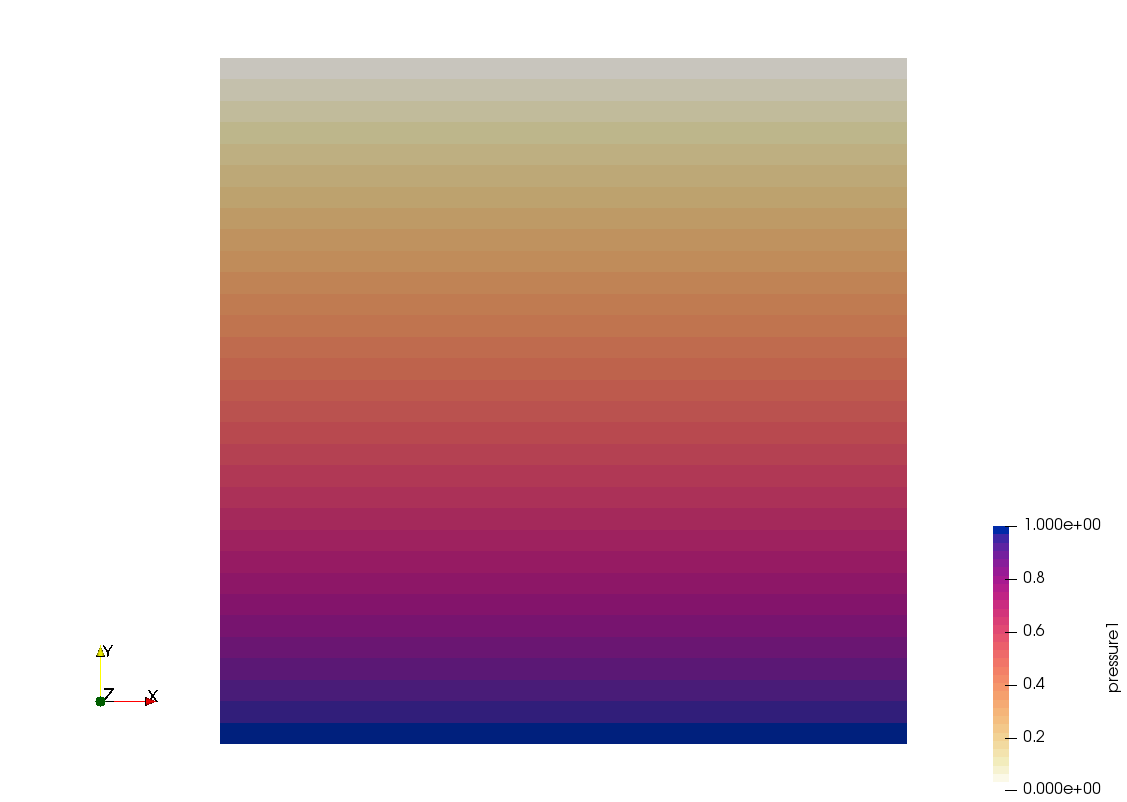
\includegraphics[width=5.7cm]{python_codes/fieldstone_119/results/exp1/p1}
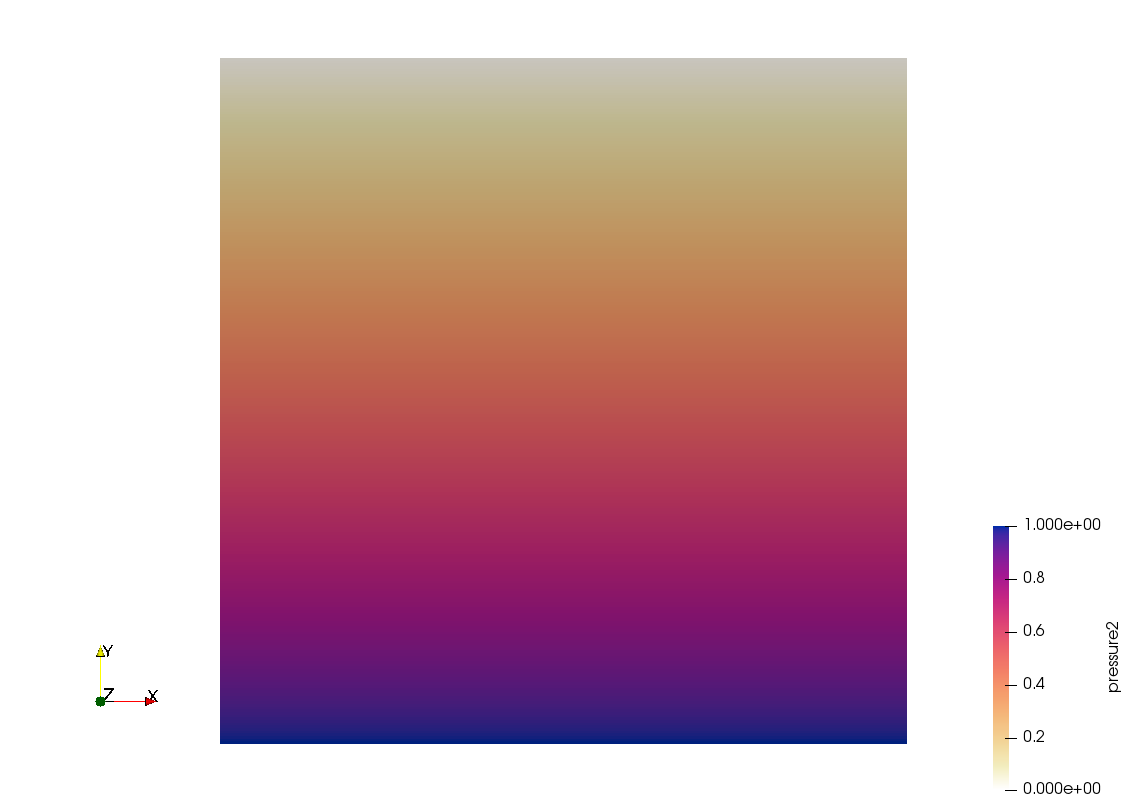
\includegraphics[width=5.7cm]{python_codes/fieldstone_119/results/exp1/p2}
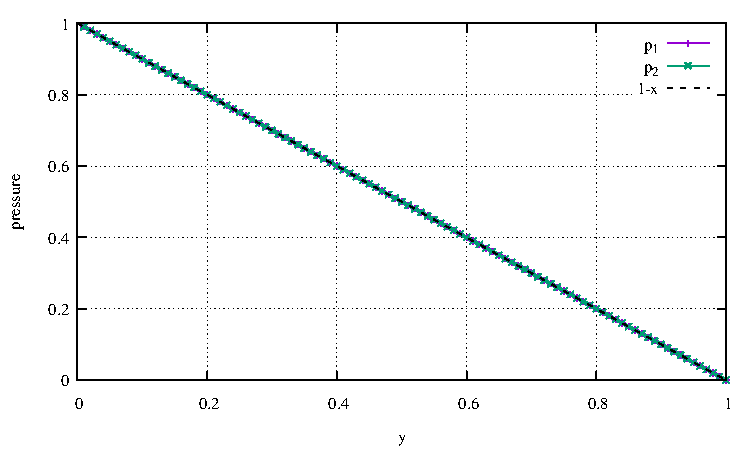
\includegraphics[width=5.7cm]{python_codes/fieldstone_119/results/exp1/profile.pdf}\\
{\captionfont Left: $p_1$; Right: $p_2$. Resolution 100$\times$100.}
\end{center}

We find that pressures $p_1$ and $p_2$ are identical.
\begin{center}
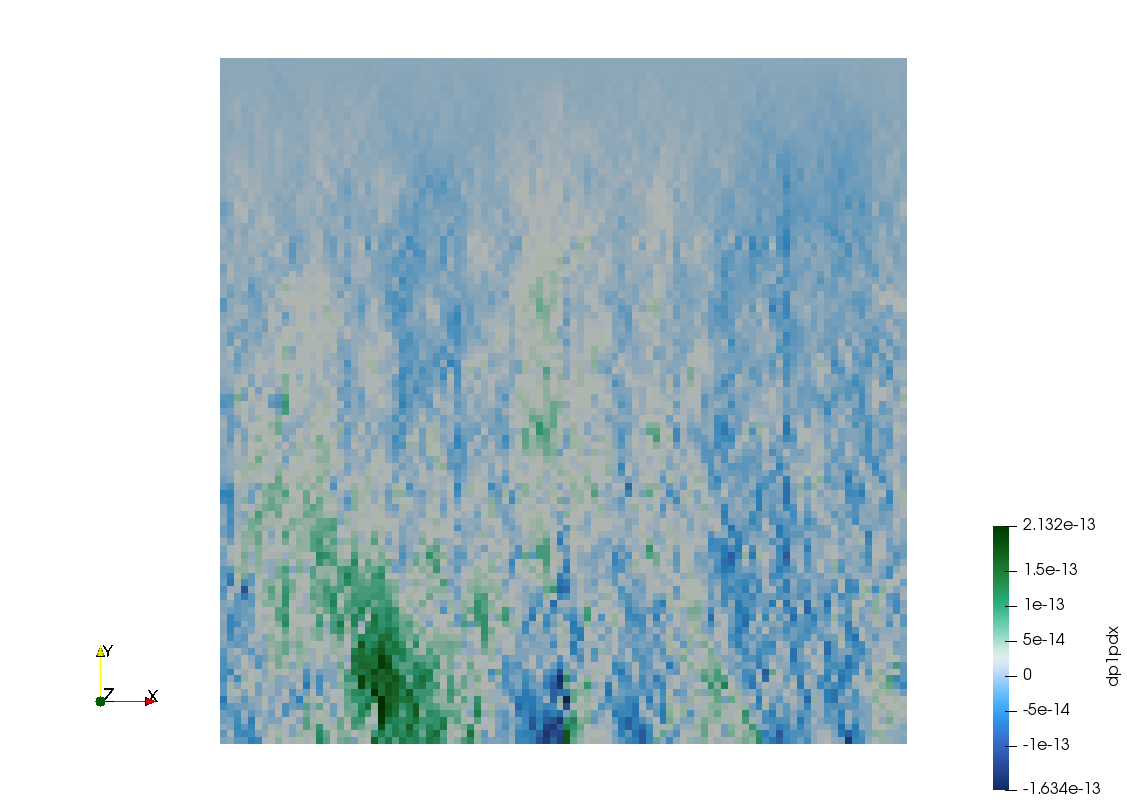
\includegraphics[width=4cm]{python_codes/fieldstone_119/results/exp1/dp1dx}
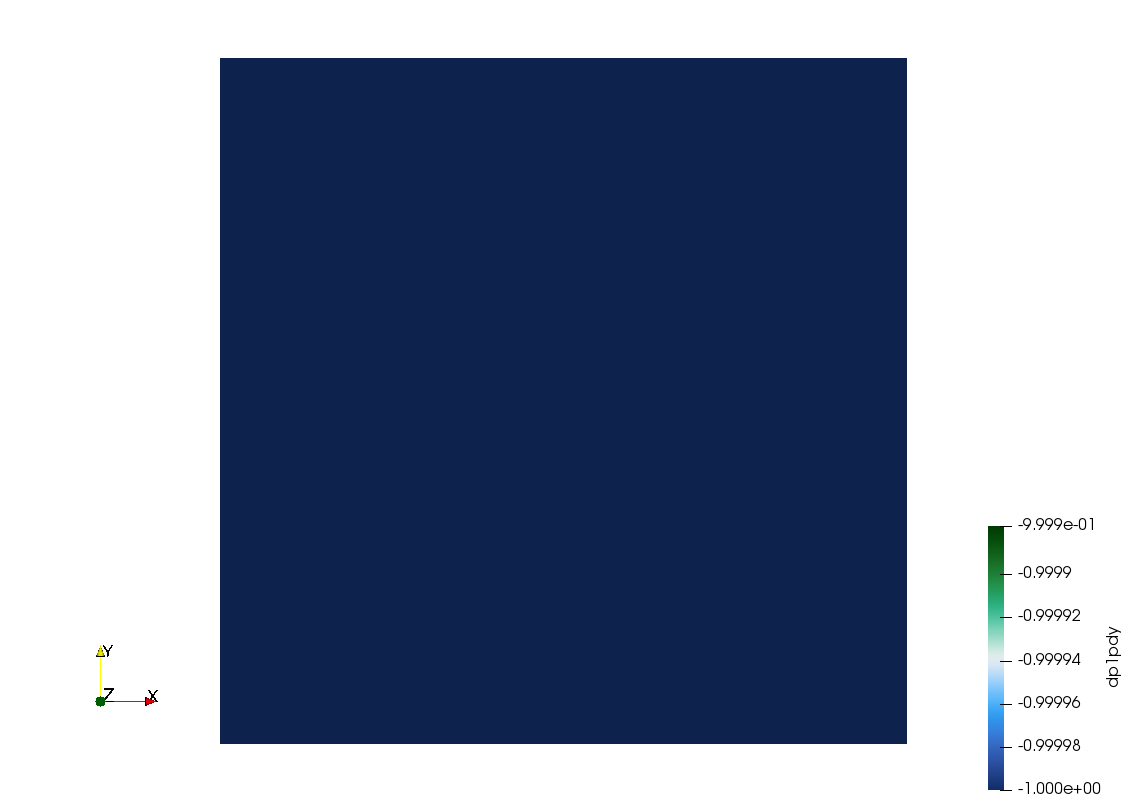
\includegraphics[width=4cm]{python_codes/fieldstone_119/results/exp1/dp1dy}
\includegraphics[width=4cm]{python_codes/fieldstone_119/results/exp1/dp2dx}
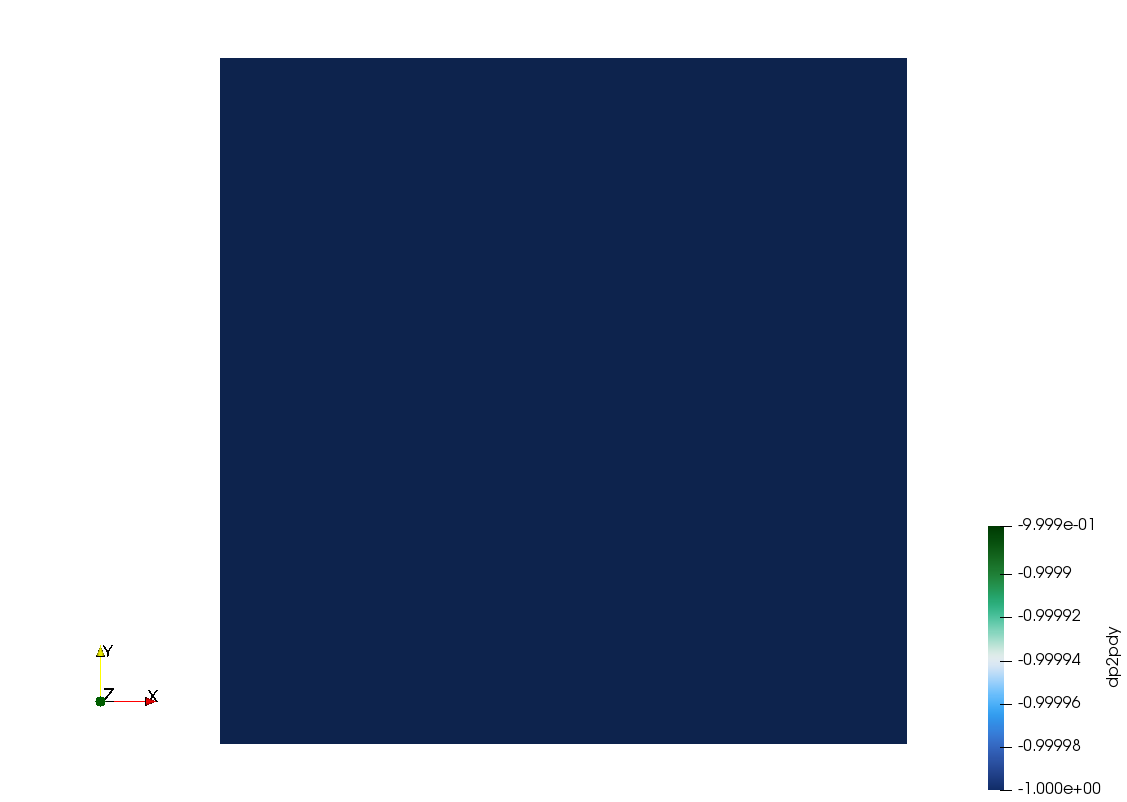
\includegraphics[width=4cm]{python_codes/fieldstone_119/results/exp1/dp2dy}\\
{\captionfont 
Pressure gradients from left to right: $\partial_xp_1$, $\partial_yp_1$, $\partial_xp_2$, $\partial_yp_2$. 
Resolution 100$\times$100.}
\end{center}

%------------------------------------------------------------------------------
\subsection*{Experiment \#2}

Same setup as Experiment \# 1, but now $\rho=1$ in the top half of the domain and $\rho=2$ in the bottom half.

\begin{center}
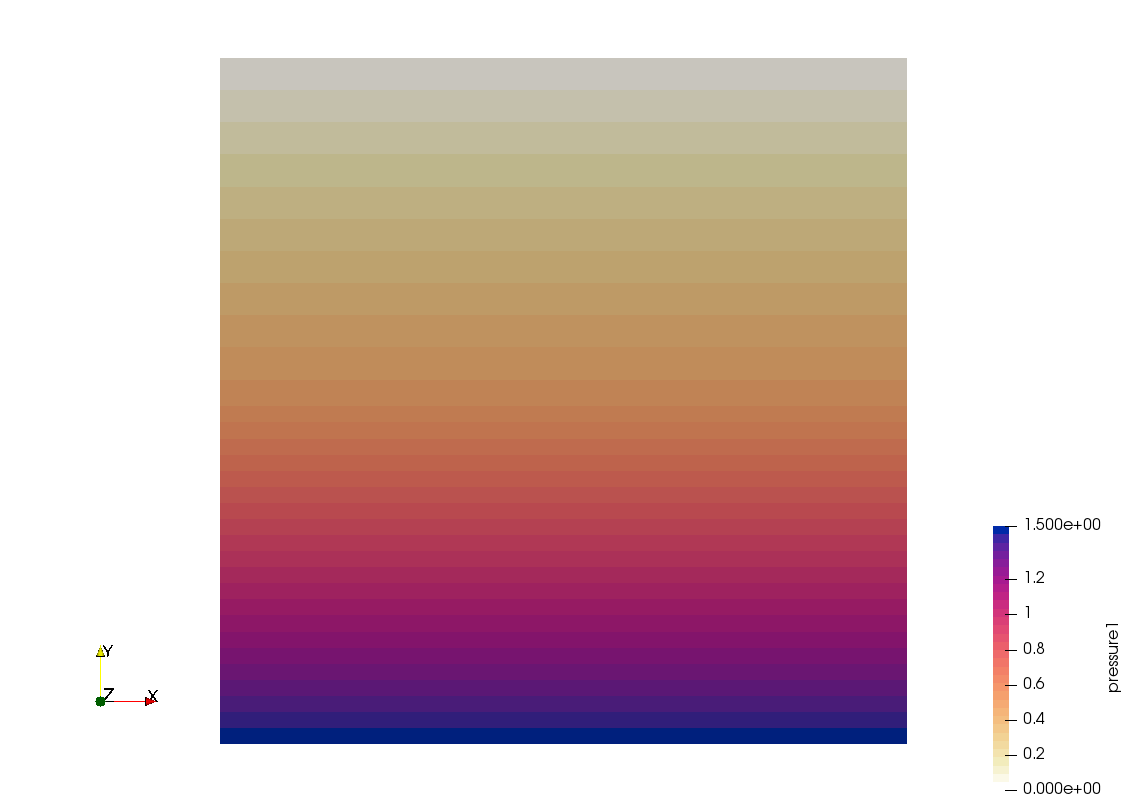
\includegraphics[width=5.7cm]{python_codes/fieldstone_119/results/exp2/p1}
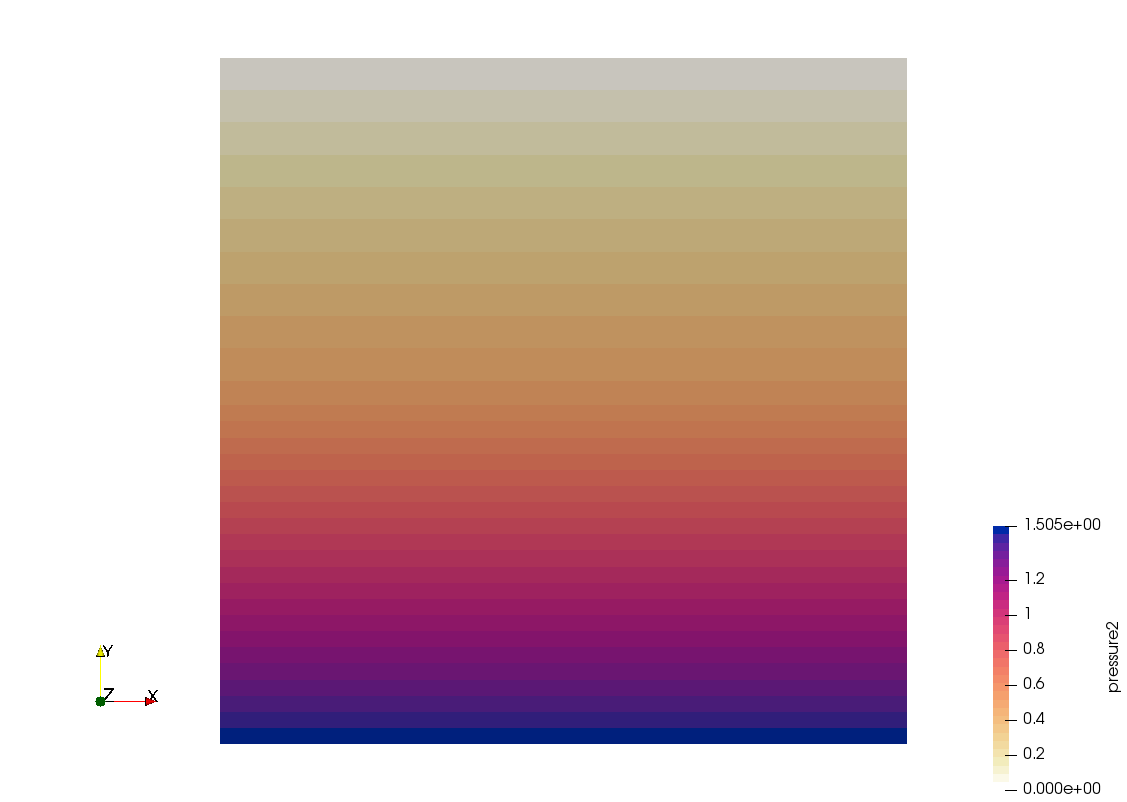
\includegraphics[width=5.7cm]{python_codes/fieldstone_119/results/exp2/p2}
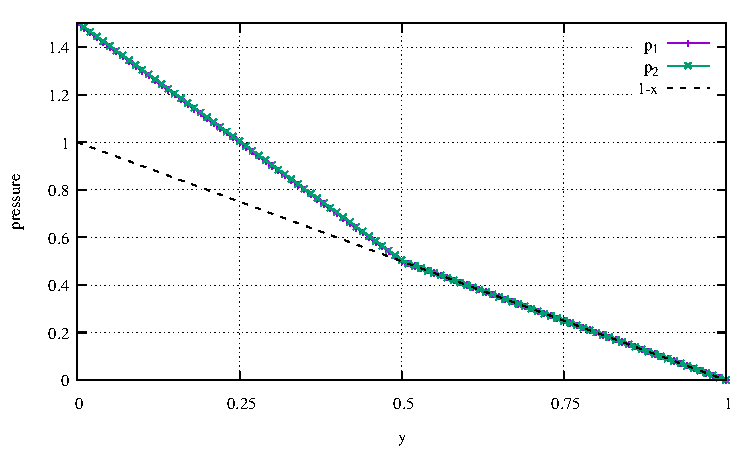
\includegraphics[width=5.7cm]{python_codes/fieldstone_119/results/exp2/profile.pdf}\\
{\captionfont Left: $p_1$; Right: $p_2$. Resolution 100$\times$100.}
\end{center}

We find that pressures $p_1$ and $p_2$ are identical.

\begin{center}
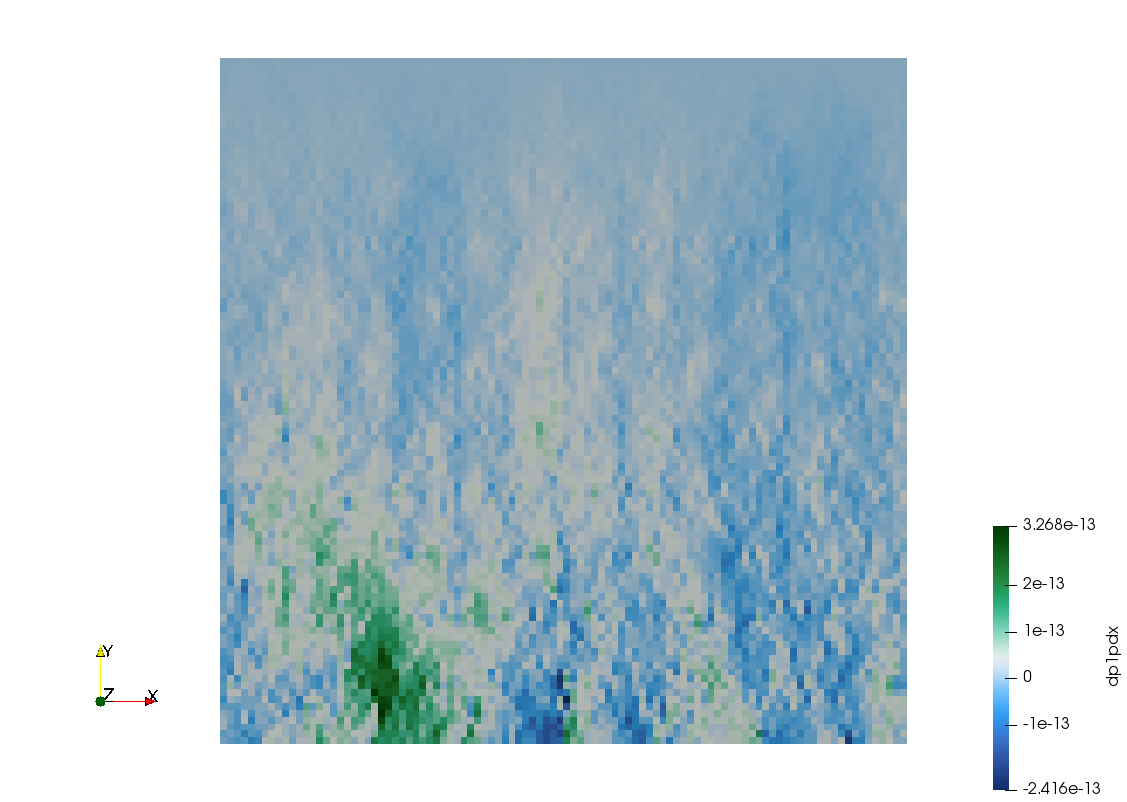
\includegraphics[width=4cm]{python_codes/fieldstone_119/results/exp2/dp1dx}
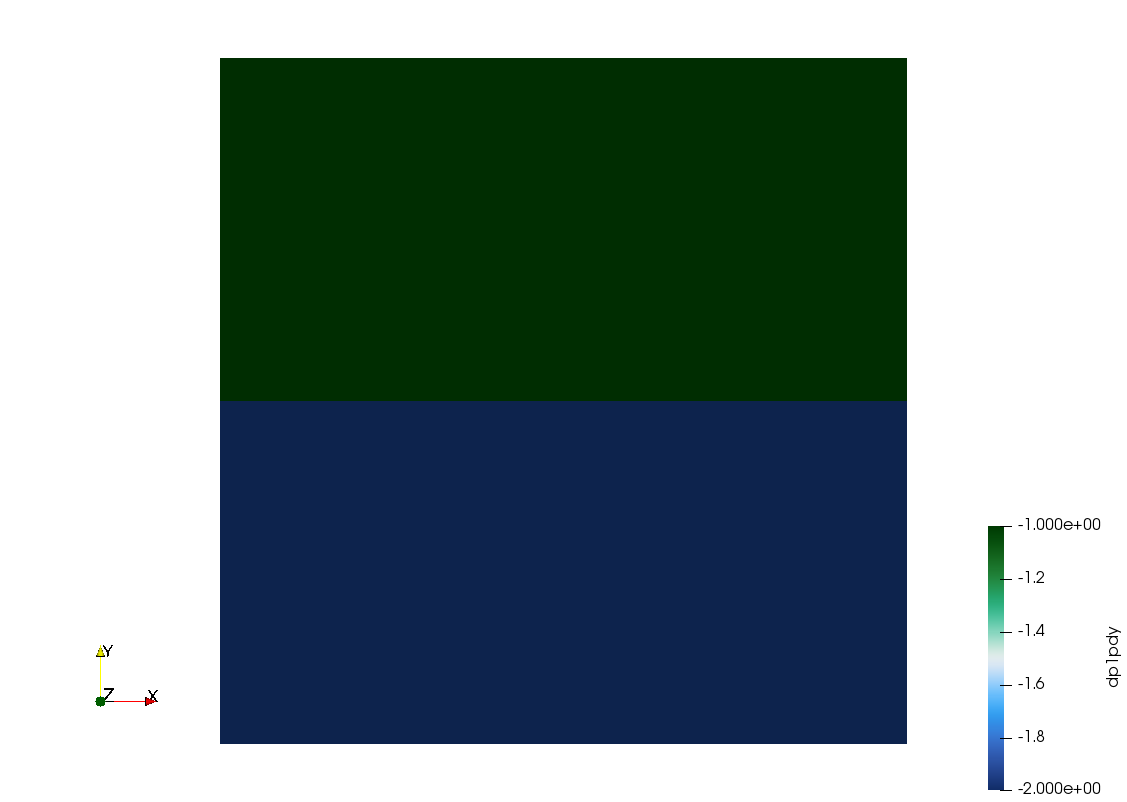
\includegraphics[width=4cm]{python_codes/fieldstone_119/results/exp2/dp1dy}
\includegraphics[width=4cm]{python_codes/fieldstone_119/results/exp2/dp2dx}
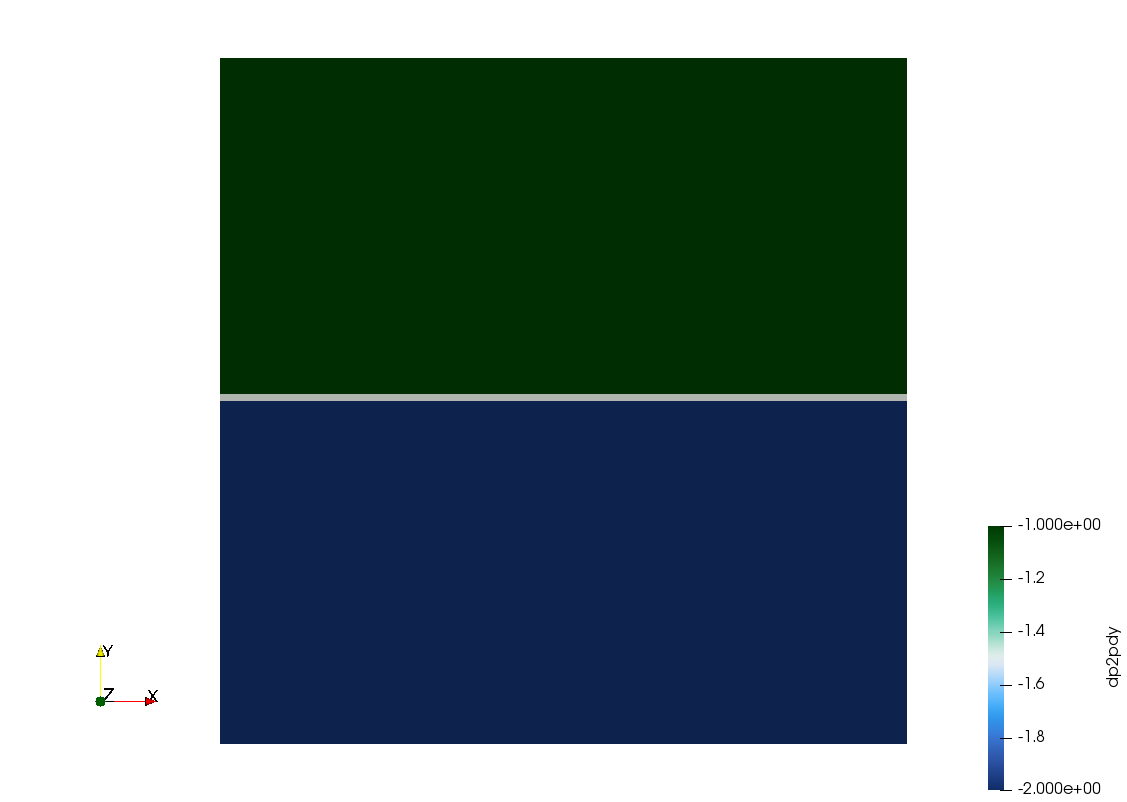
\includegraphics[width=4cm]{python_codes/fieldstone_119/results/exp2/dp2dy}\\
{\captionfont 
Pressure gradients from left to right: $\partial_xp_1$, $\partial_yp_1$, $\partial_xp_2$, $\partial_yp_2$. 
Resolution 100$\times$100.}
\end{center}

\newpage
%------------------------------------------------------------------------------
\subsection*{Experiment \#3}

Same setup as Experiment \# 1, but now $\rho=1$ in the left half of the domain and $\rho=2$ in the right half.

\begin{center}
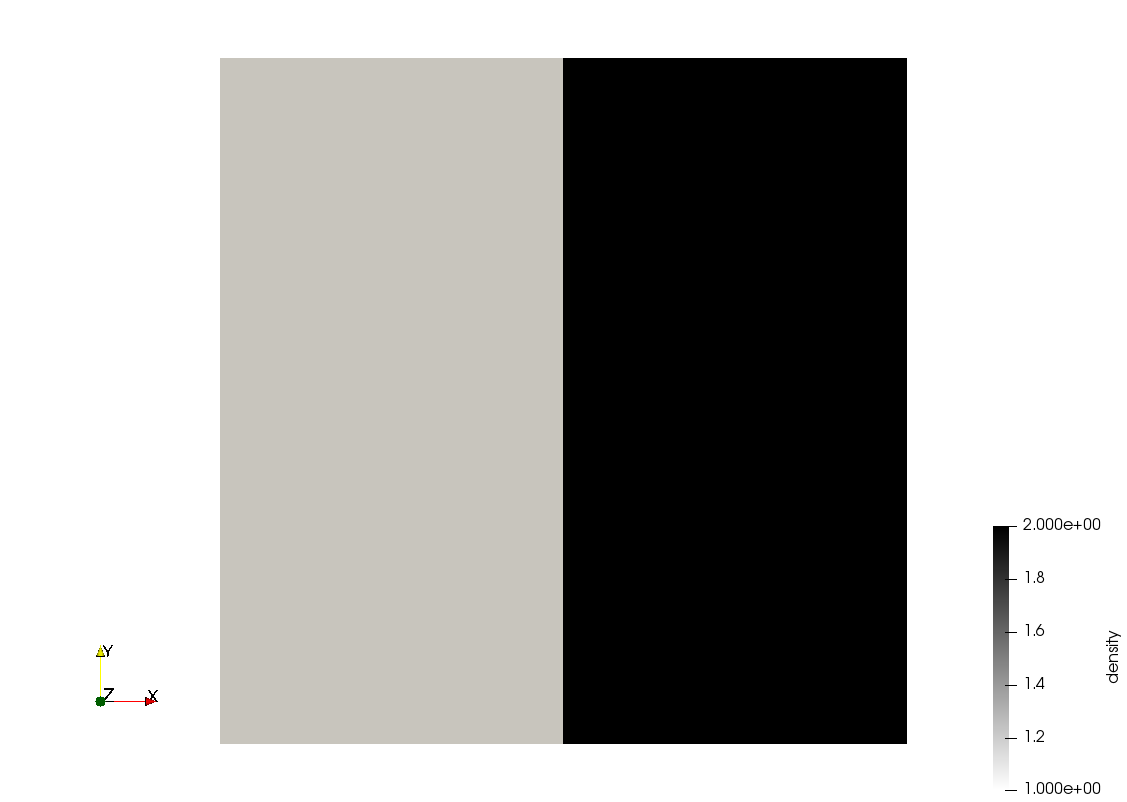
\includegraphics[width=5.6cm]{python_codes/fieldstone_119/results/exp3/rho}
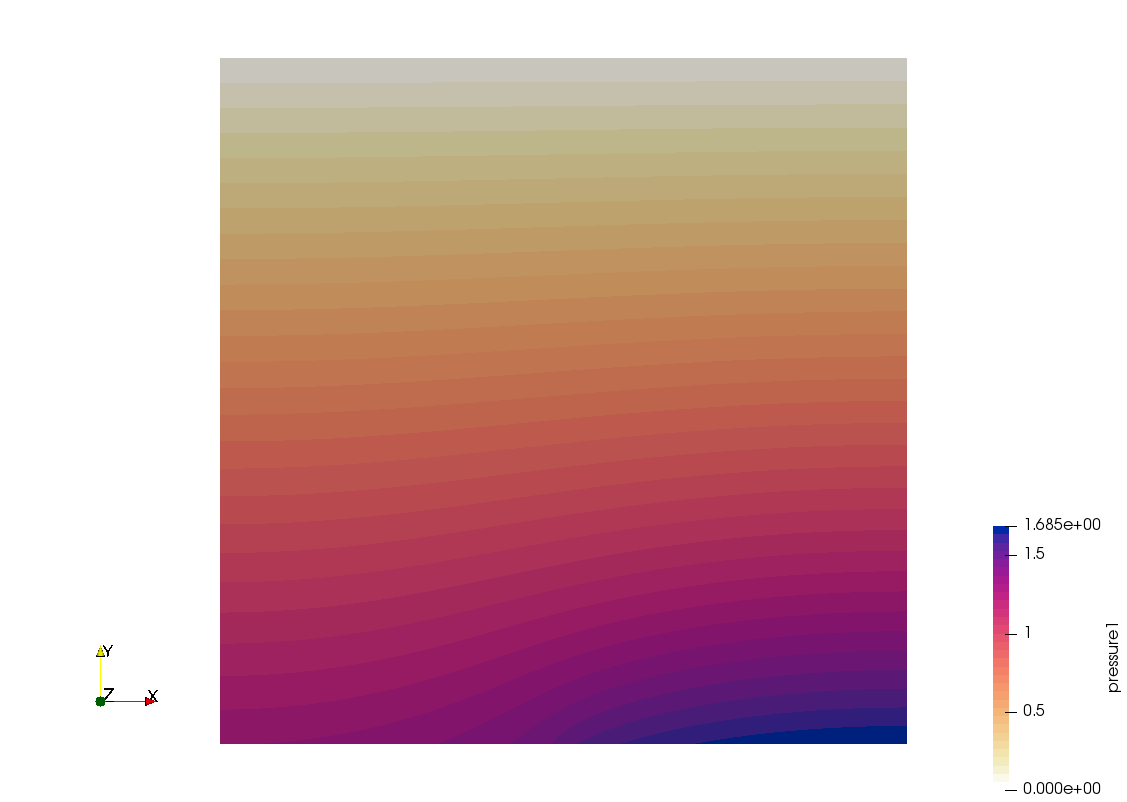
\includegraphics[width=5.6cm]{python_codes/fieldstone_119/results/exp3/p1}
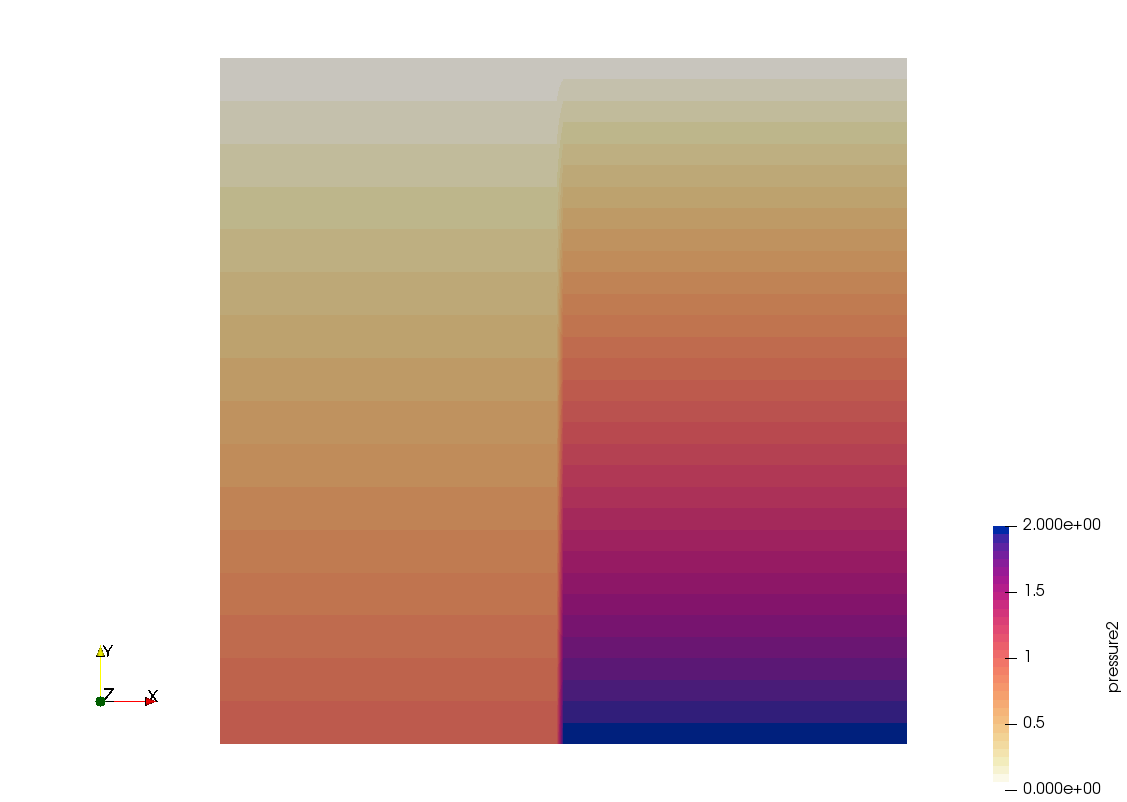
\includegraphics[width=5.6cm]{python_codes/fieldstone_119/results/exp3/p2}\\
{\captionfont Left: density; middle: $p_1$; Right: $p_2$. Resolution 100$\times$100.}
\end{center}

\begin{center}
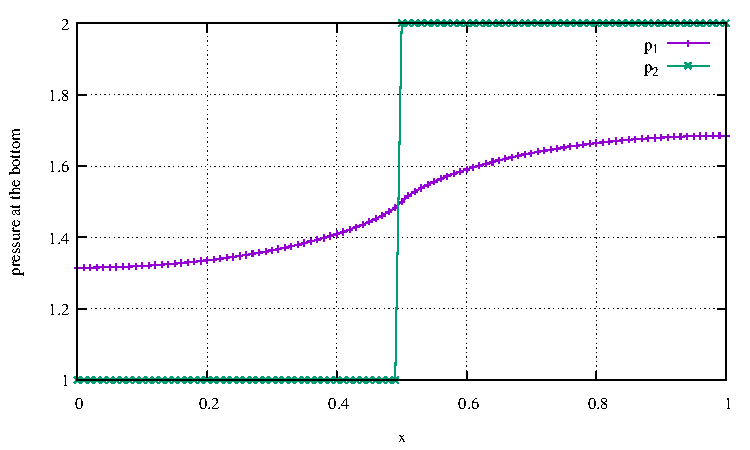
\includegraphics[width=5.7cm]{python_codes/fieldstone_119/results/exp3/bottom}
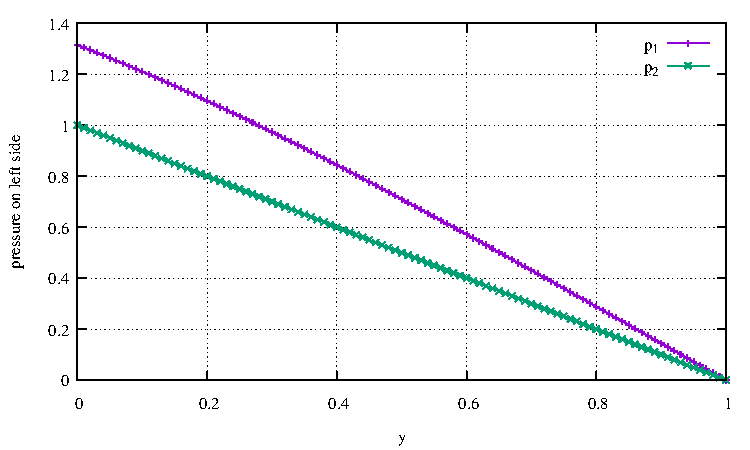
\includegraphics[width=5.7cm]{python_codes/fieldstone_119/results/exp3/left}
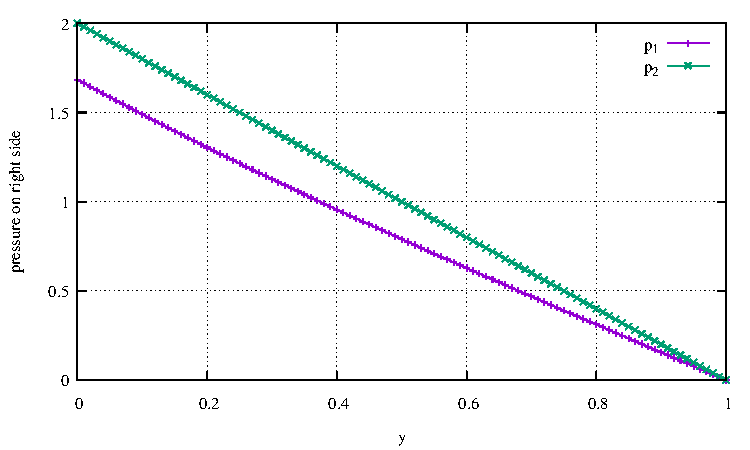
\includegraphics[width=5.7cm]{python_codes/fieldstone_119/results/exp3/right}\\
{\captionfont Pressure profiles at the bottom, left and right boundaries}
\end{center}

We find that pressures $p_1$ and $p_2$ are very different (pattern and amplitude). 

\begin{center}
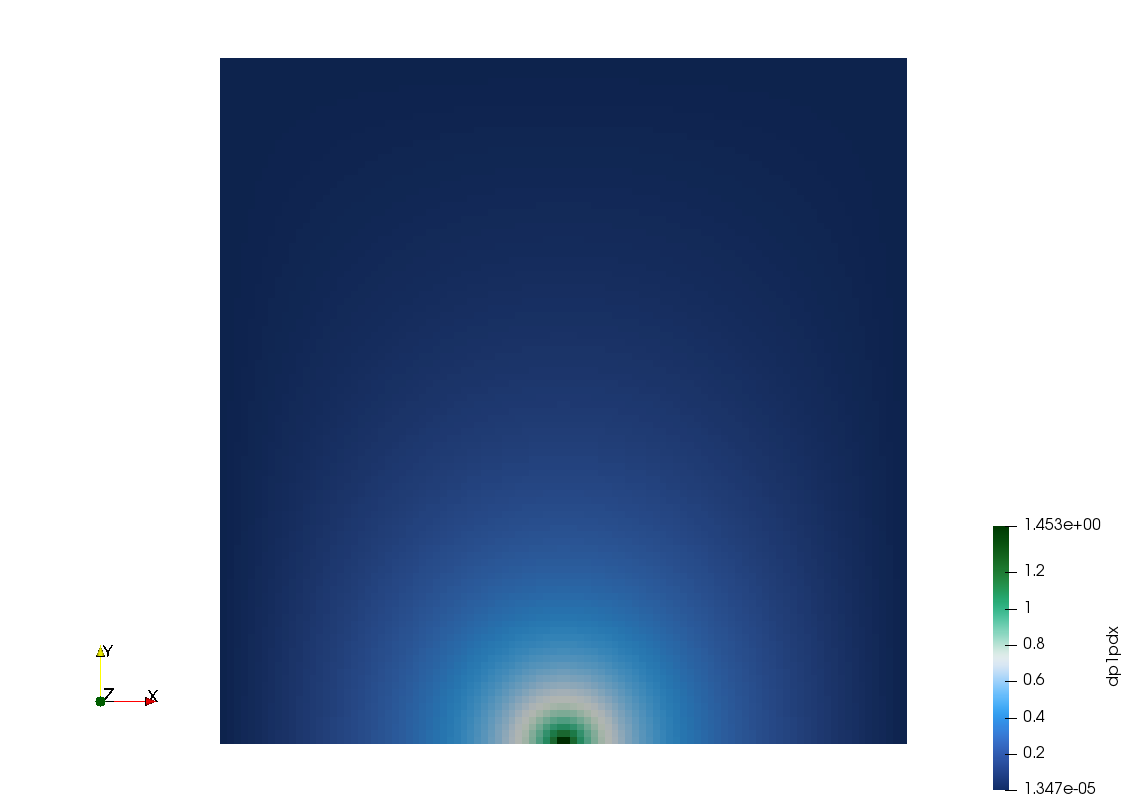
\includegraphics[width=4.2cm]{python_codes/fieldstone_119/results/exp3/dp1dx}
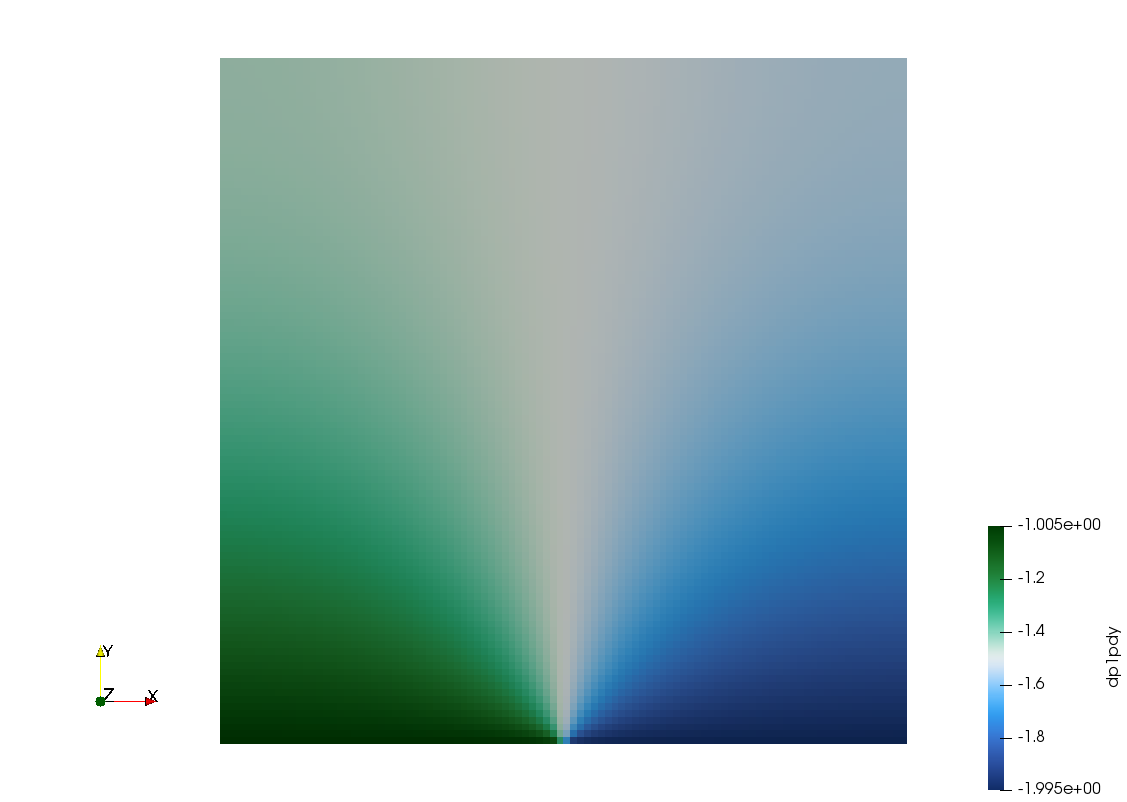
\includegraphics[width=4.2cm]{python_codes/fieldstone_119/results/exp3/dp1dy}
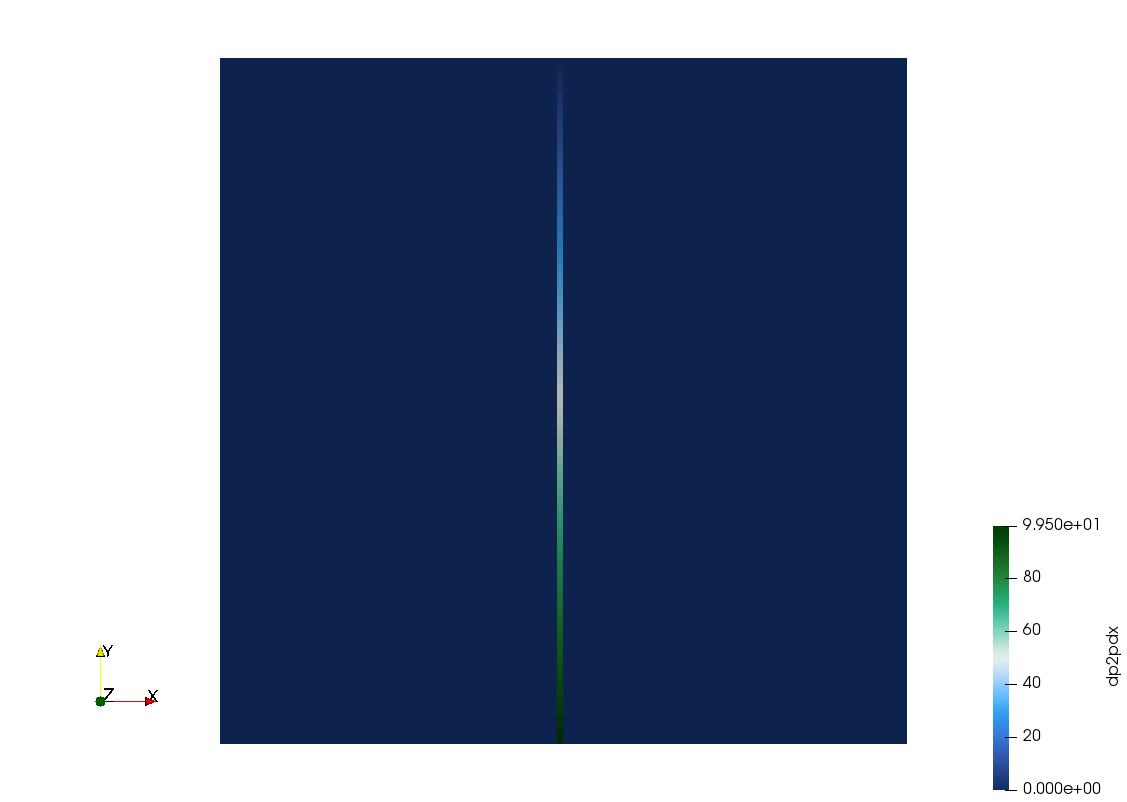
\includegraphics[width=4.2cm]{python_codes/fieldstone_119/results/exp3/dp2dx}
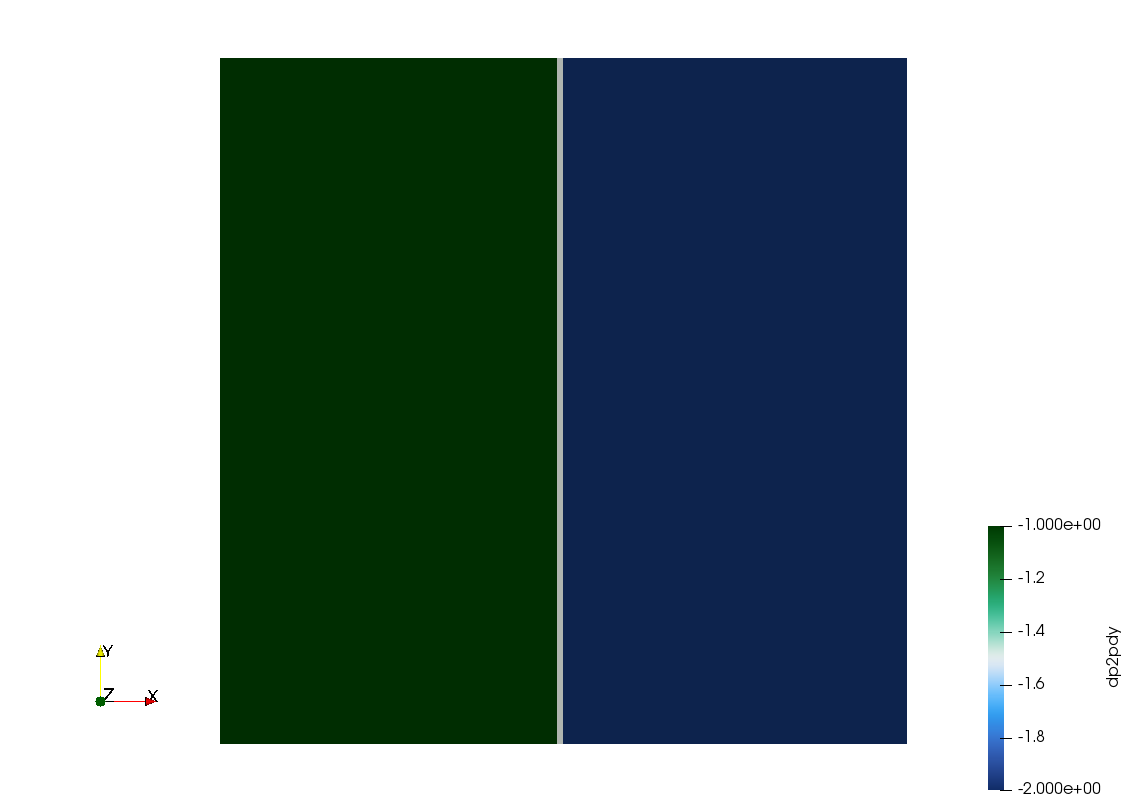
\includegraphics[width=4.2cm]{python_codes/fieldstone_119/results/exp3/dp2dy}\\
{\captionfont Pressure gradients from left to right: $\partial_xp_1$, $\partial_yp_1$, $\partial_xp_2$, $\partial_yp_2$. 
Resolution 100$\times$100.}
\end{center}

Obviously we do not have $\vec{\nabla}p=-\rho\vec{g}$ for the pressure obtained with 
the Poisson equation!

\newpage
%------------------------------------------------------------------------------
\subsection*{Experiment \#4}

In this experiment the density is 1 except in a centered disc of radius 0.25 in which it is 2, 
and $g=10$. I have approached A. Jourdon and asked him to carry out this experiment 
with the code used in his paper. 

\begin{center}
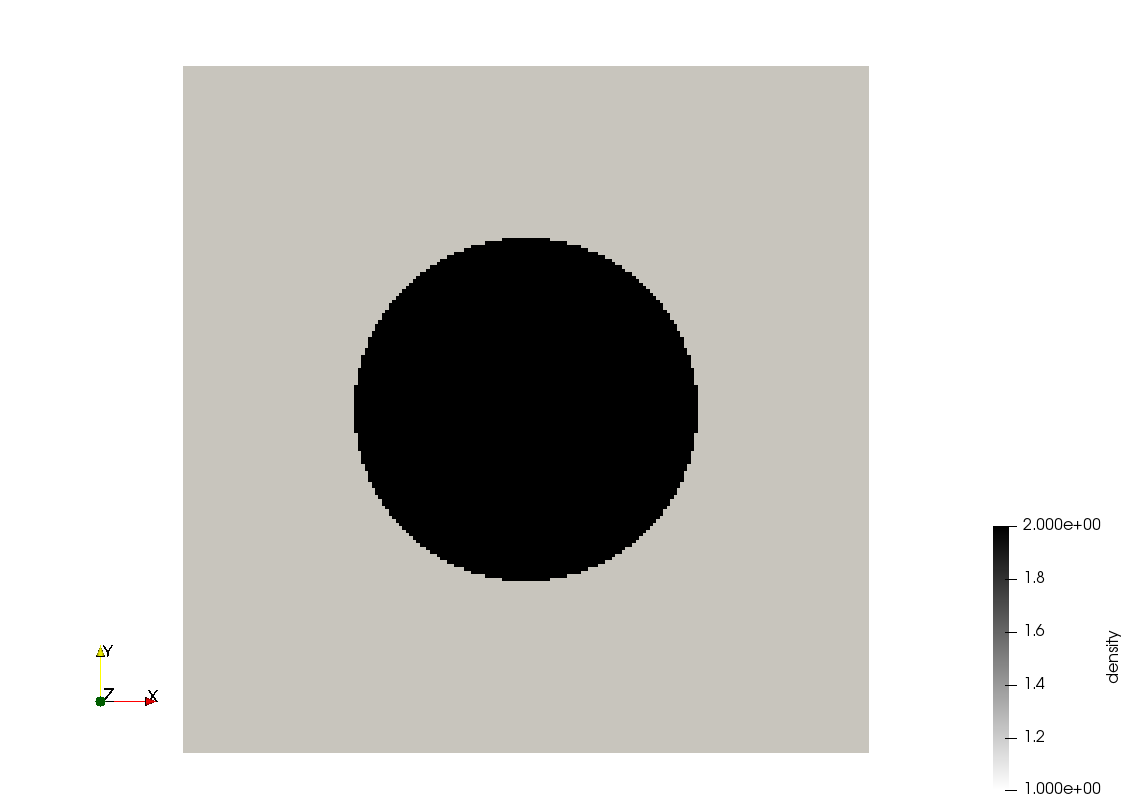
\includegraphics[width=7cm]{python_codes/fieldstone_119/results/exp4/rho}
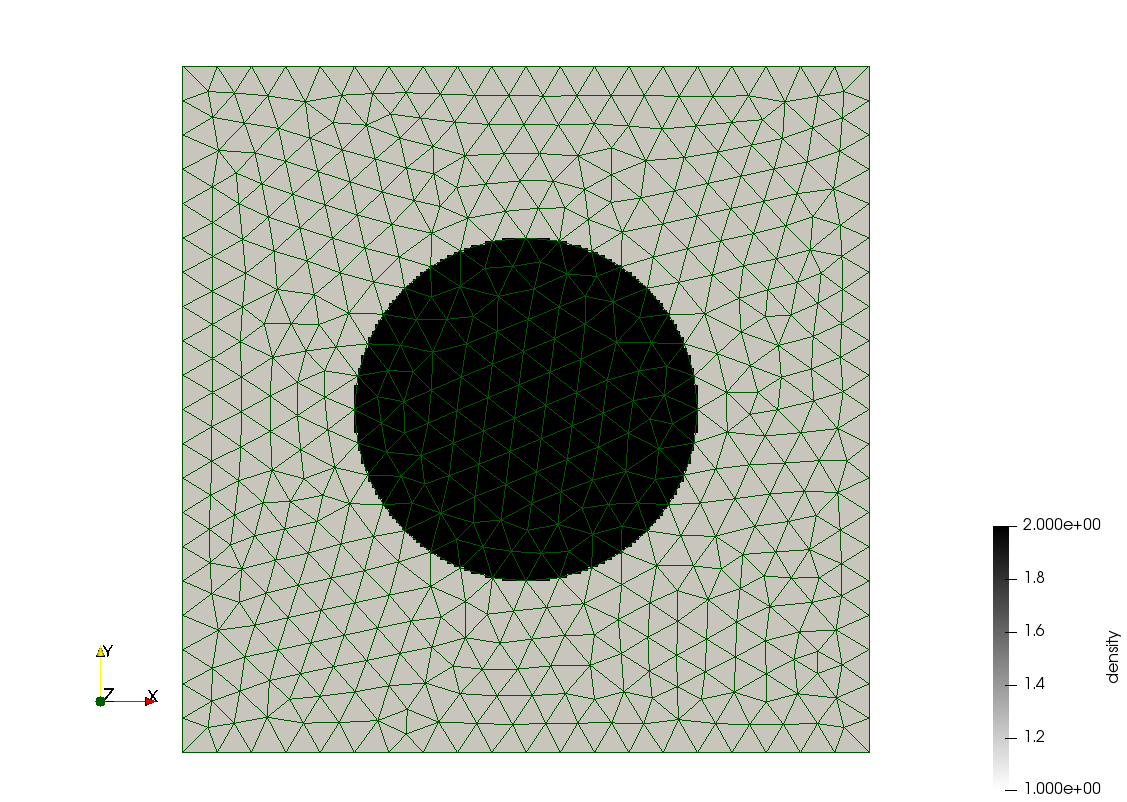
\includegraphics[width=7cm]{python_codes/fieldstone_119/results/exp4/rho_joma22_mesh}\\
{\captionfont Left: density field on 200x200 mesh. right: mesh used by Jourdon with 
my density field superimposed.}
\end{center}

\begin{center}
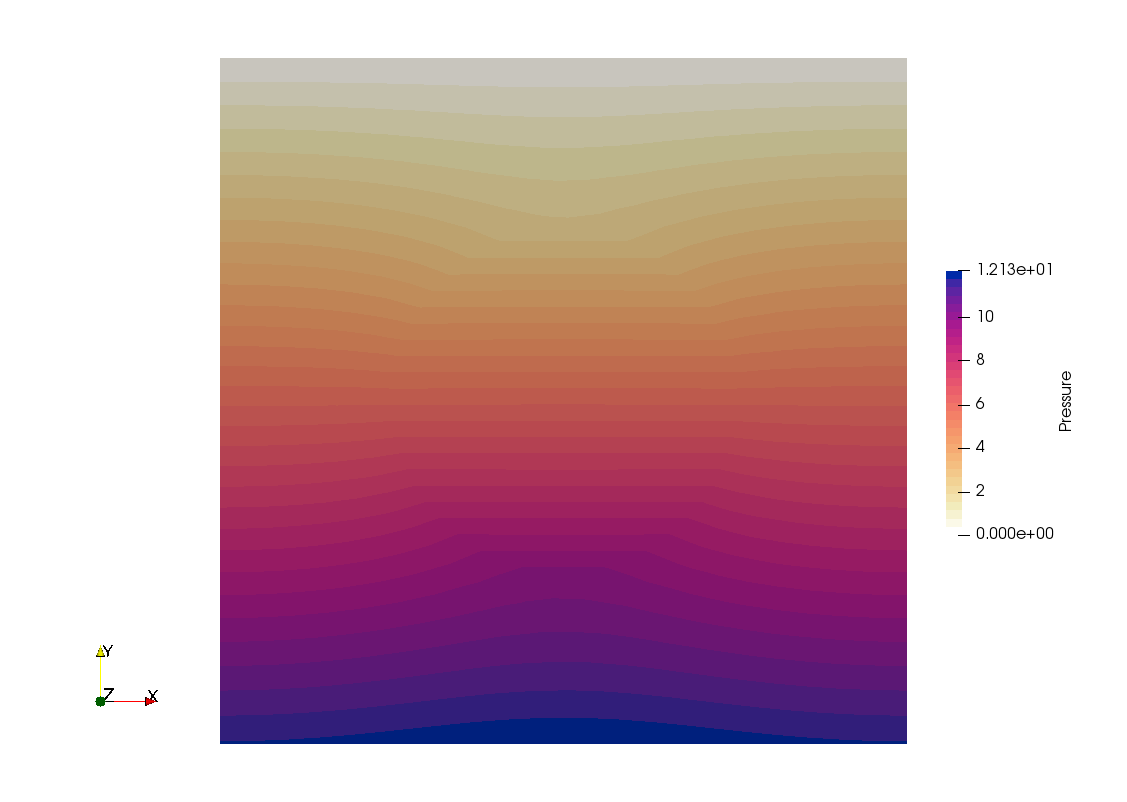
\includegraphics[width=5.7cm]{python_codes/fieldstone_119/results/exp4/p_joma22}
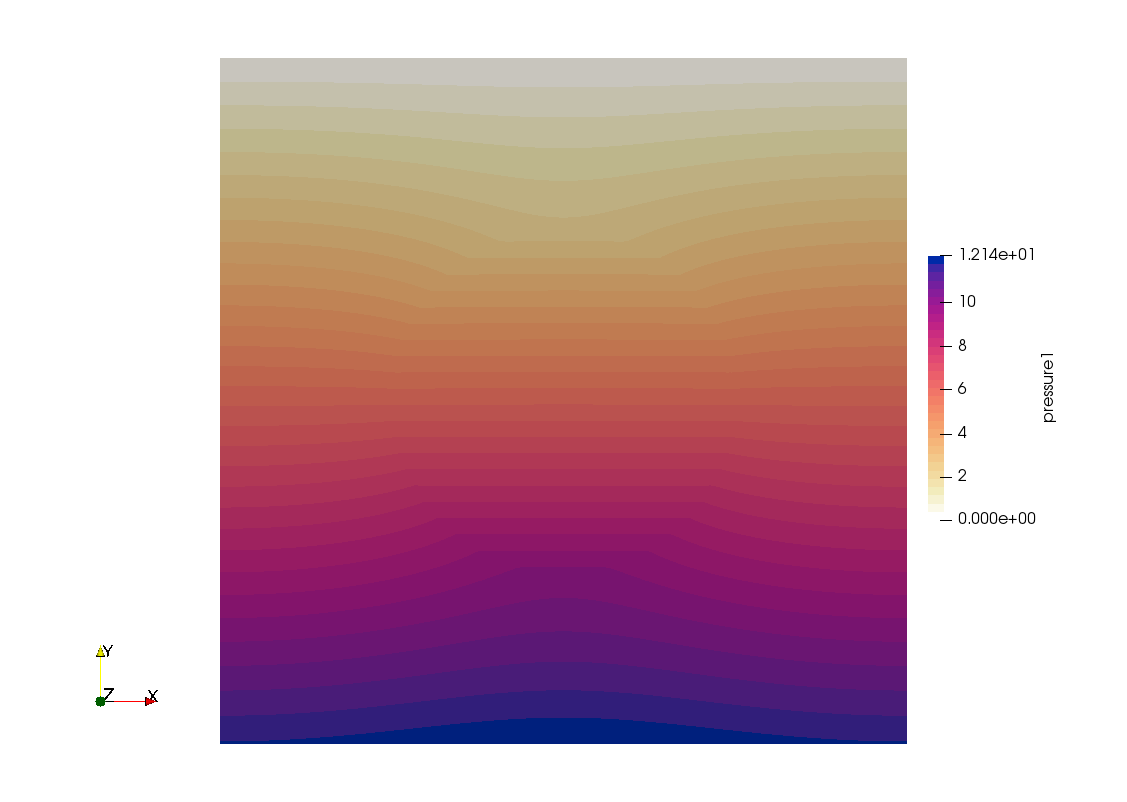
\includegraphics[width=5.7cm]{python_codes/fieldstone_119/results/exp4/p1}
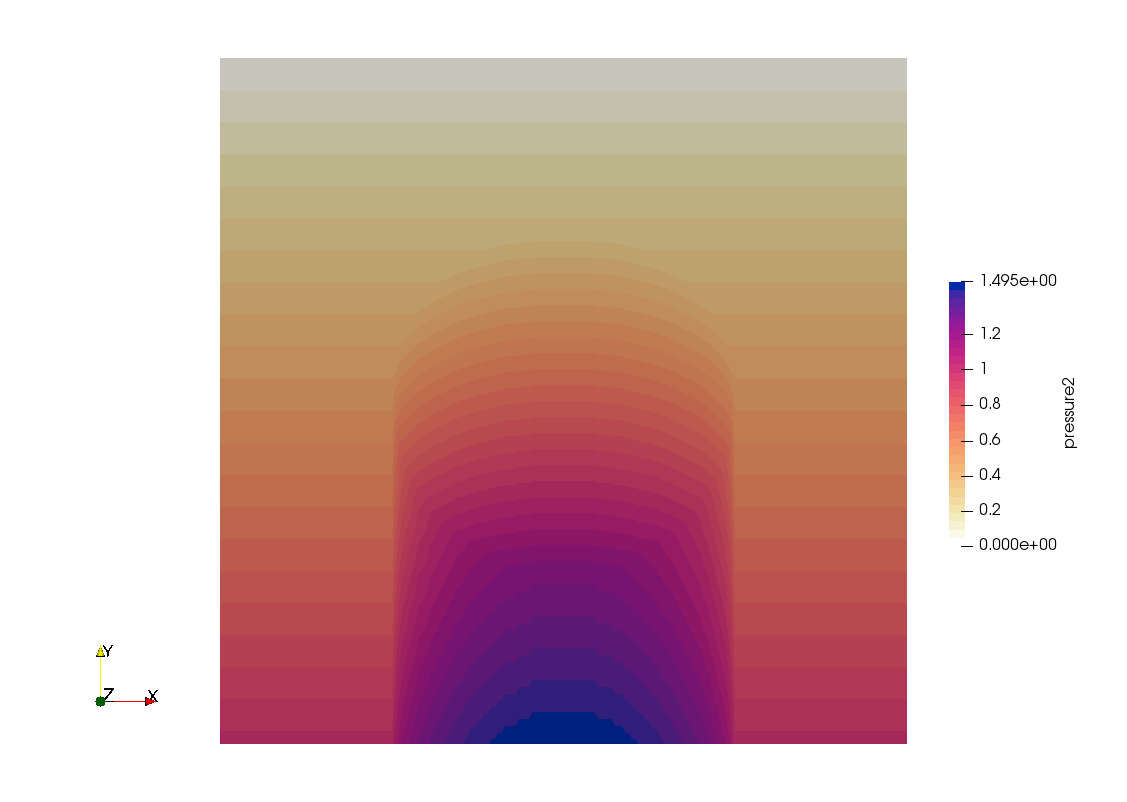
\includegraphics[width=5.7cm]{python_codes/fieldstone_119/results/exp4/p2}\\
{\captionfont Left: pressure from Jourdon; Middle: $p_1$; Right: $p_2$. Resolution 200$\times$200.}
\end{center}

\begin{center}
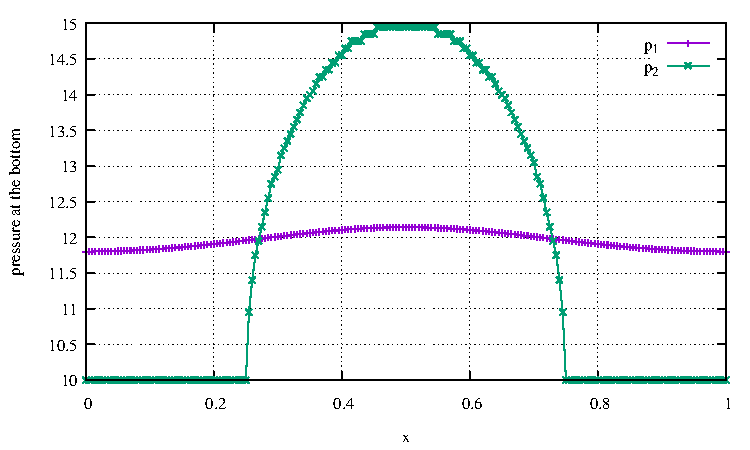
\includegraphics[width=7.5cm]{python_codes/fieldstone_119/results/exp4/bottom}
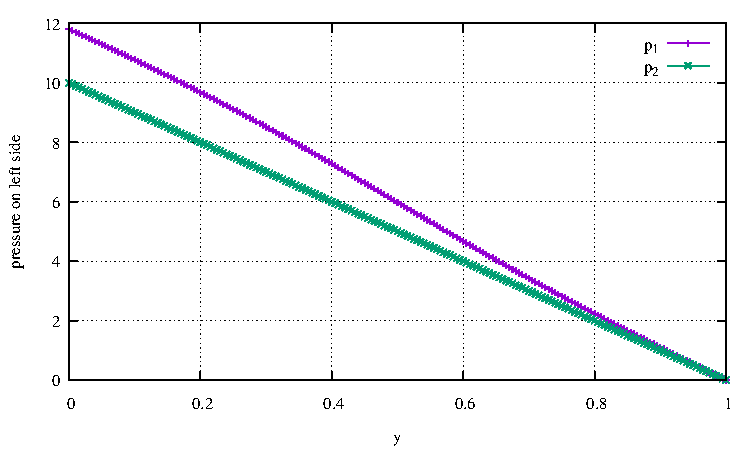
\includegraphics[width=7.5cm]{python_codes/fieldstone_119/results/exp4/left}\\
{\captionfont Pressures $p_1$ and $p_2$ at the bottom and left boundary.}
\end{center}

We find that pressures $p_1$ and $p_2$ are again very different (pattern and amplitude), but 
we find that $p_1$ and the results sent by Jourdon are identical (which validates my implementation):

\begin{center}
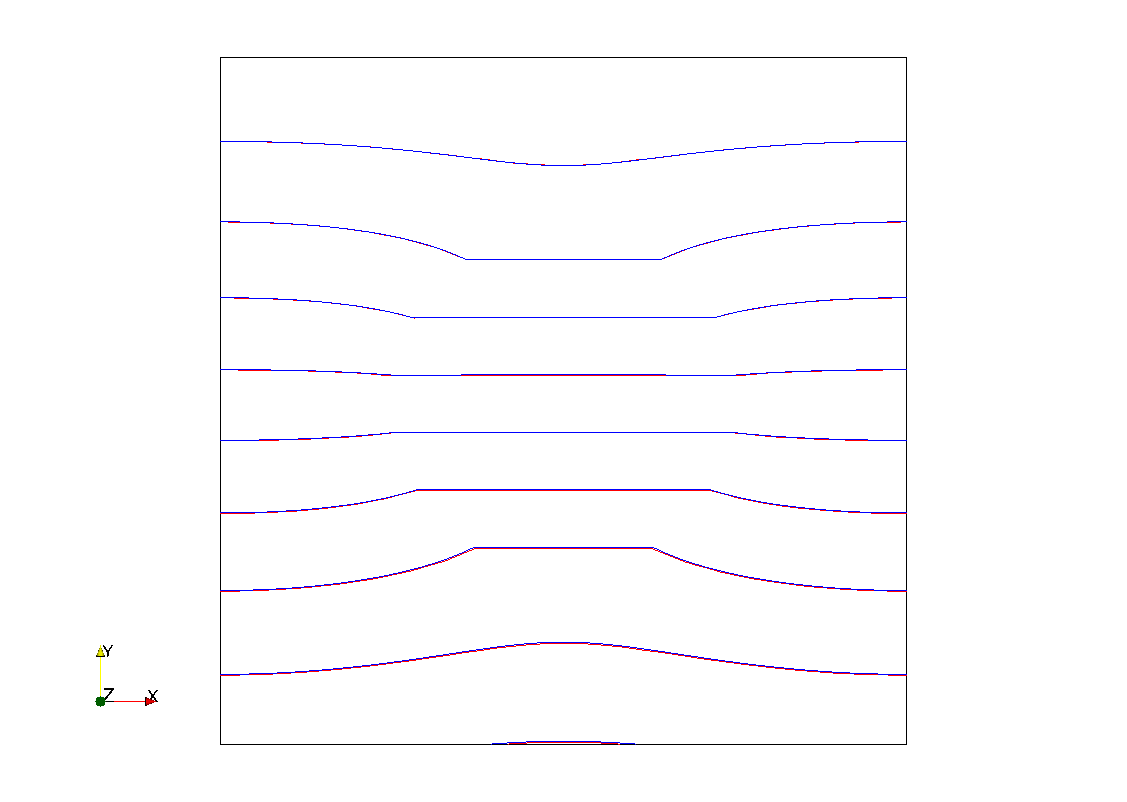
\includegraphics[width=7cm]{python_codes/fieldstone_119/results/exp4/p1_both}\\
{\captionfont Pressure isocontours for both pressures obtained with this \stone and Jourdon's code.}
\end{center}
 
\begin{center}
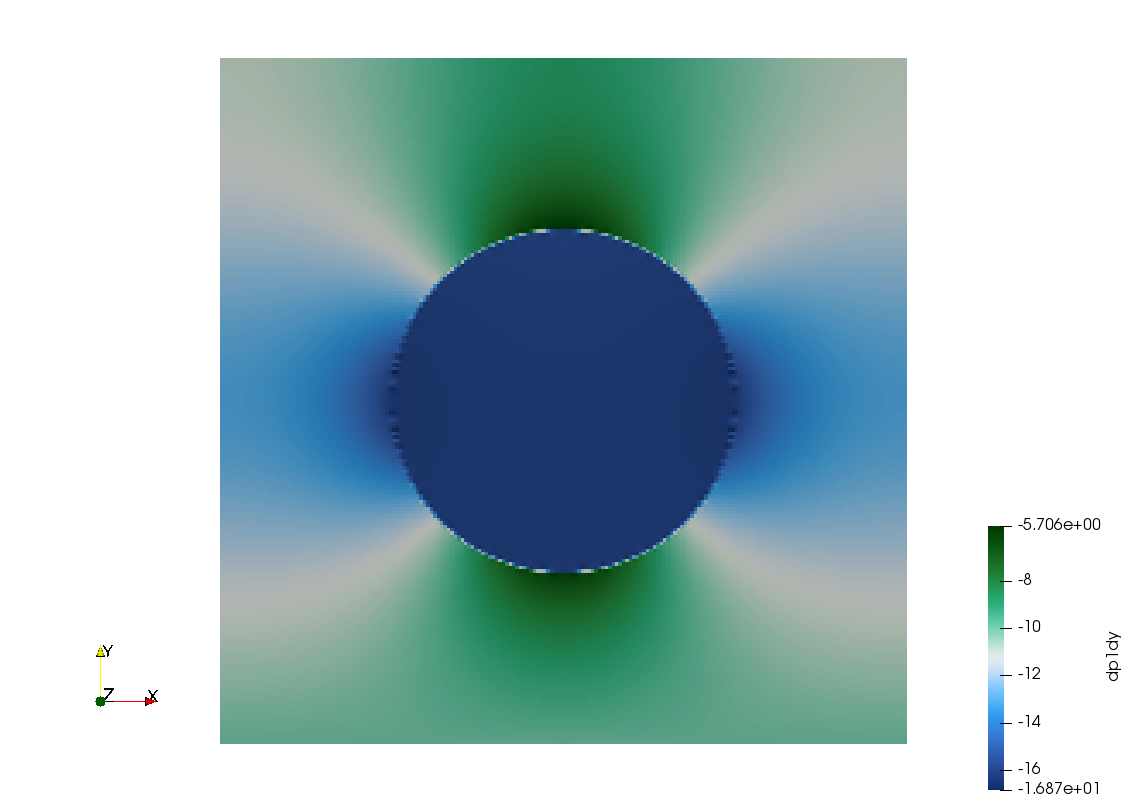
\includegraphics[width=7cm]{python_codes/fieldstone_119/results/exp4/dp1dy}
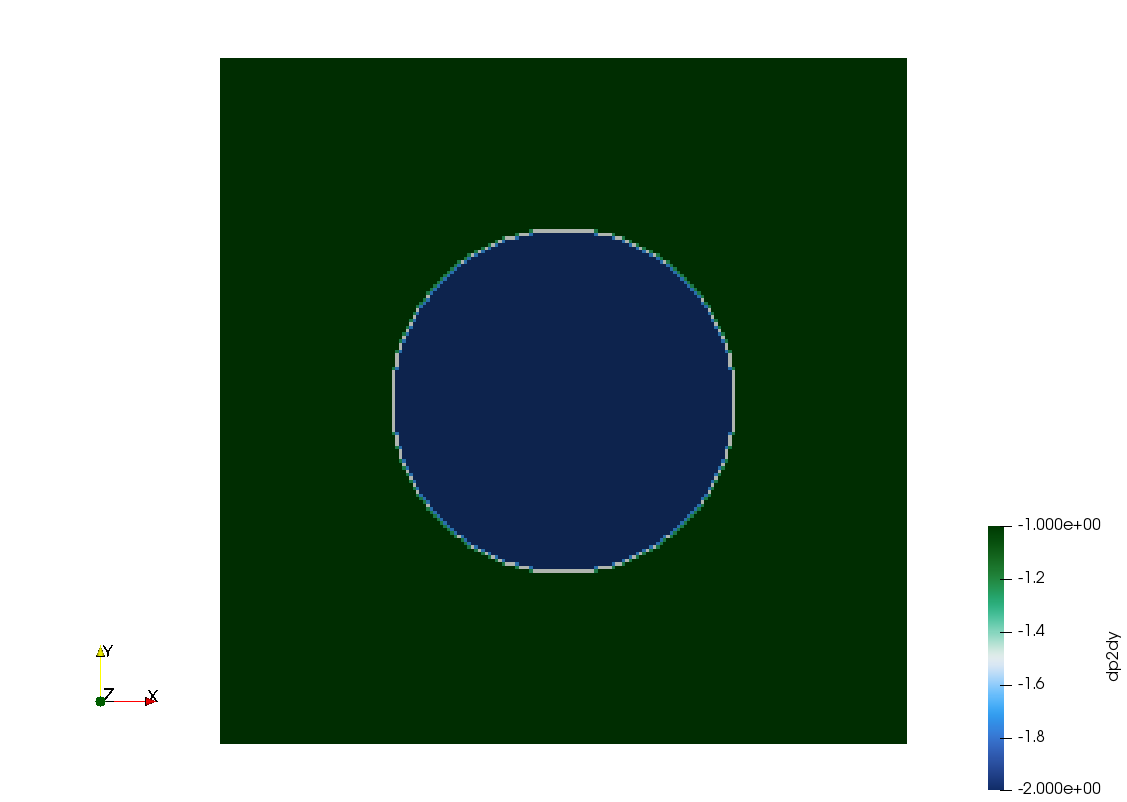
\includegraphics[width=7cm]{python_codes/fieldstone_119/results/exp4/dp2dy}\\
{\captionfont Pressure gradients. Left: $\partial_yp_1$; Right: $\partial_yp_2$. Resolution 200$\times$200.}
\end{center}

Obviously we here again do not have $\vec{\nabla}p=-\rho\vec{g}$ for the pressure obtained with 
the Poisson equation!
The pressure at the bottom for $x<0.25$ should be constant and equal to 10, but this is not 
the case for the Poisson pressure, so it is not a lithostatic pressure. Only $p_2$ is. 





